\documentclass{classeENS}
\usepackage{lipsum}

\title{Template rapport ENS } %Titre du fichier



\begin{document}

%----------- Informations du rapport ---------

\titre{Study of the Stanford CoreNLP Natural Language Processing Toolkit} %Titre du fichier .pdf
\departement{Master MVA} 
\matiere{Fundamentals of Reproducible Research and Free Software} 
\motif{First report}

\enseignant{Miguel Colom\\ \\} %Nom de l'enseignant
%\tuteurpcp{}
\eleves{Alice Valença De Lorenci \\ Clément Weinreich \\ Thibault Robine} %Nom des élèves

%----------- Initialisation -------------------
        
\fairemarges %Afficher les marges
\fairepagedegarde %Créer la page 
\tableofcontents 


\newpage

\section{Introduction}\label{sec:introduction} 

The objective of this project is to study the Stanford CoreNLP toolkit, a Java-based open source software project developed by the Stanford Natural Language Processing Group, that provides linguistic annotations \cite{CoreNLP}. 

Originally designed in 2006, this Java toolkit was developed in order to tie multiple language analysis components together. The main motivations of the CoreNLP toolkit architecture was to create a straightforward and lightweight framework in plain Java that efficiently provides linguistic annotations while hiding component differences behind a unified and easy-to-understand interface. In 2009, the Stanford NLP Group extended their software to make it more easily usable by a broader range of users. They provided a command-line interface and added the possibility of writing annotations with different formats, such as the widely used XML format. Finally, the project was released as a free open source software in 2010. The original architecture is still the basis of today’s CoreNLP toolkit \cite{ToolkitPaper}. 

In essence, it consists in a natural language processing toolkit that takes in raw text and generates a variety of linguistic annotations, such as parts of speech, named entities, dependencies and co references, as illustrated on Fig. \ref{fig:annotation examples}. It is widely used by the NLP community not only for research but also in the industry and public organizations. Available on GitHub \cite{CoreNLPGit}, there is an active community of developers maintaining the project (9.2k stars and 171 currently open issues). Their website also allows users to test the toolkit through an interactive demo \cite{CoreNLPDemo}. 

\begin{figure}[H] 
    \center
    \subfigure[Parts of speech annotations.]{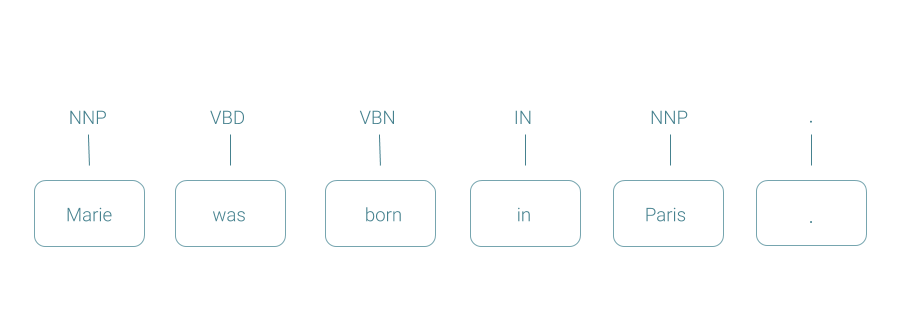
\includegraphics[width=0.45\linewidth]{figs/pos.png}}
    \quad
    \subfigure[Named entities annotations.]{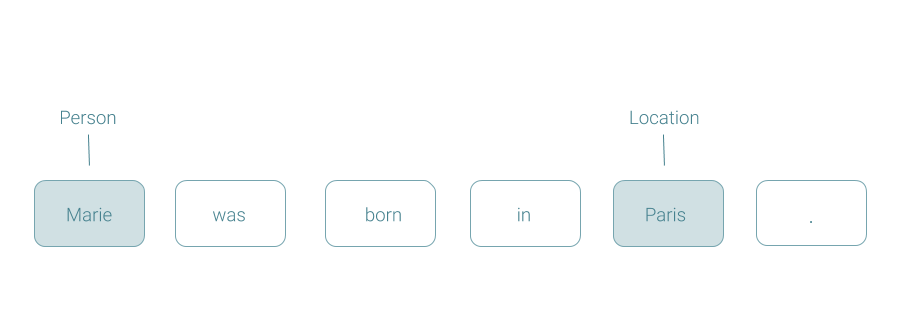
\includegraphics[width=0.45\linewidth]{figs/ner.png}}
    \\
    \subfigure[Dependency parses annotations.]{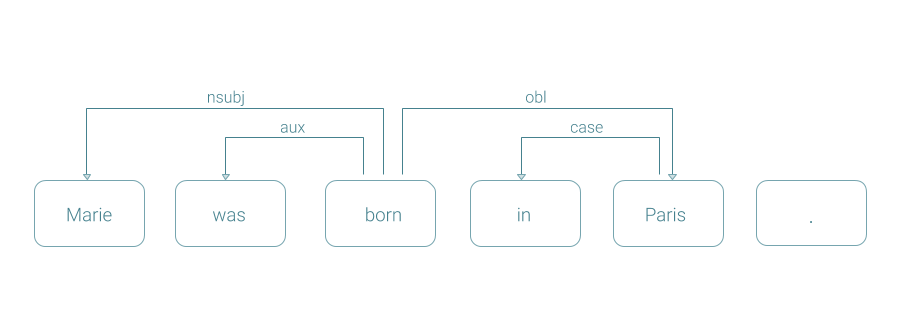
\includegraphics[width=0.45\linewidth]{figs/depparse.png}}
    \quad
    \subfigure[Co reference annotations.]{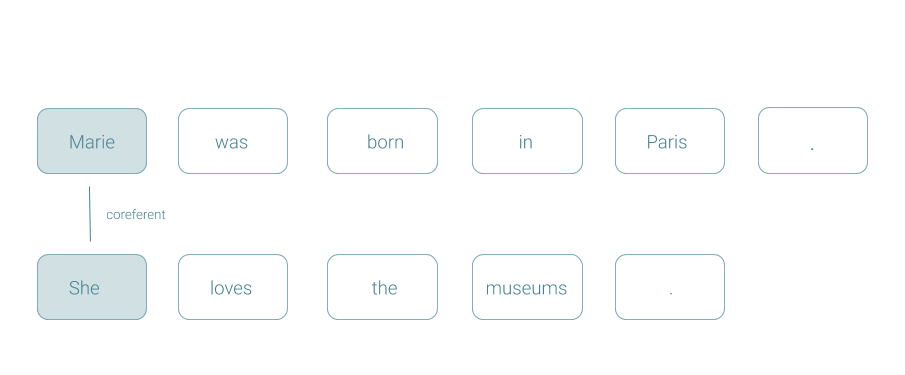
\includegraphics[width=0.45\linewidth]{figs/coref.png}}
    \caption{Illustration of the different linguistic annotations supported by CoreNLP. Source: \cite{CoreNLP}.}
    \label{fig:annotation examples}
\end{figure}


This first report aims to study the software through several angles. Its main users and target domain will be described. Also, the economic model of the project will be dissected. Finally, the software license and the resulting usage possibilities will be analyzed. 

\section{Target users and domain}\label{sec:target}

Stanford CoreNLP was initially designed in 2006 for internal use by the Stanford Natural Language Processing Group. Since then, the system was extended and released as open source software in 2010, targeting the broader NLP research community as well as commercial and governmental users of NLP tools \cite{ToolkitPaper}.

The interest of Stanford CoreNLP with respect to other NLP frameworks is that it provides a simple unified Java API, making it easily accessible to a wide range of users. For example, although it does provide multi-thread support for a single machine, it does not propose multiple machine scale-out solutions, relegating this task to the organizations. The result is a software that is easily installed and understood and that, if necessary, can be adapted by the organization to their preferred scale-out solution. Furthermore, it doesn't require GPU and is well optimized which makes it well adapted to simple NLP use cases with reduced footprint. Therefore, users with minimal knowledge in NLP can benefit from the easy-to-understand interface of CoreNLP to use it for their applications. 

One of the main use cases of Stanford CoreNLP is the development of chat bots. For instance the open conversational AI platform Tock (The Open Conversation Kit) uses CoreNLP \cite{Tock}. As stated on their websites, the Tock platform is used by companies and governmental organizations such as SNCF, EDF or AlloCovid for their conversational agents.

In addition, the theoretical aspects behind Stanford CoreNLP are accessible at a graduate level thanks to the abundant documentation on the subject. The original paper of the project also makes reference to the papers used to implement the algorithms in the toolkit. Along with the source code and the documentation (available on \cite{CoreNLPUsage}), it is possible to study in detail how the toolkit works, which allows a wide range of users to understand the project in order to use it and contribute to it.

% \section{A brief overview of the theory}

% For a better grasp of the interest and applications of the toolkit, the Stanford Classifier, one of the algorithms implemented by the toolkit, will be briefly described. This algorithm is a supervised algorithm for text classification, there is no pre-trained model and the Stanford CoreNLP offers a toolkit to train the users model.

% The first step of the algorithm is the featurization. The algorithm will go through each example $(h',t')$ in the training data set, and will generate a feature function of the following form:
% \begin{equation}
% \text{TO DO}
% \end{equation}
% Where $w'_{\pm k}$ is the k\textsuperscript{th} word in $h'$ and $t'$ the associated class. It will then associate a weight to each feature function.

% The goal of the algorithm is to compute the probability of a text being in a class with the exponential family.
% \begin{equation}
% \text{TO DO}
% \end{equation}

% It then uses an optimization algorithm in order to find the weight that maximizes conditional entropy. It is important to note that this optimization problem is convex.
% \begin{equation}
% \text{TO DO}
% \end{equation}

% A new example can then be classified by calculating the probability of it being in each class.

\section{Economic Model}\label{sec:economic model}

The economic model employed by the Stanford CoreNLP software is that of dual licensing \cite{CoreNLP}. As will be detailed in the next session, the software is licensed under the GNU General Public License, that is a free-software license. However, this license requires that any derivative works (software based on CoreNLP) must also be licensed under the GPL, which means they must be open source. Thus, it does not allow its use in proprietary software distributed to others. In order to circunvent this, Stanford also offers the software under a commercial license, that appeals to distributors of proprietary software. 

So, while the GPL requires open sourcing any derivative works, the dual licensing model allows for the use of Stanford CoreNLP in proprietary software by obtaining a separate, proprietary license from the developers. This enables users to choose between open-source and proprietary use of the software based on their specific needs. Therefore the software generates revenue through companies buying a commercial license for proprietary use.

 It is worthwhile mentioning that the Stanford NLP Group also welcomes donations to support the maintenance of the toolkit \cite{CoreNLP}. Since we do not have access to the amount or origin of the donations it wasn't possible to determine whether it characterizes a corporate development and distribution economic model. The fact however that two of the co-authors of the CoreNLP are researchers at IBM and Prismatic Inc. suggests that those companies might have funded the development of the project.

 \section{Licensing and free software}\label{sec:licesing}

The Stanford CoreNLP toolkit is licensed under the GNU General Public License v3, or a later version. Specifically, while all of the Stanford NLP code is GPL v2+, CoreNLP incorporates some Apache-licensed libraries, which results in an overall licensing of GPL v3+. In this section, we first analyze the license, and then explain the possibilities for the development of the project from the point of view of developers and users, according to their business model. In particular, we analyze the license through the perspective of the four freedoms of free software as defined by the FSF (Free Software Foundation) \cite{FSFfreedoms}. 
 
The key points of the GPLv3+ license that legally binds CoreNLP and its usage are :
\begin{itemize}
    \item \textbf{Copyleft:} The GPLv3+ is a copyleft license, which means that the source code must be available to others, so anyone can use, modify and distribute the software as well. It also ensures that any derivative works of CoreNLP also remains open-source.
    
    \item \textbf{Compatibility:} This license is designed to be compatible with GPLv3 and any future versions of the GPL.

    \item \textbf{User freedoms:} GPLv3+ ensures that users have the right to study, modify and share the software CoreNLP (freedoms 1 and 2 of free softwares \cite{FSFfreedoms}). It also includes provisions to protect against digital rights management restrictions.

    \item \textbf{Patent Provisions:} The license provides protection for users against patent claims that could arise from the use of CoreLNP.  It means that if a distributor of CoreNLP brings a patent lawsuit against a user for using CoreNLP, their rights to distribute the software under the GPL license can be terminated.
    
    \item \textbf{Community and Contributions:} Being open source, Stanford CoreNLP benefits from contributions and collaboration from the community of users and developers. If any user makes improvements or fixes to the software, they can contribute to the project by releasing their improvements to the public, so that the whole community benefits (freedom 3 of free softwares \cite{FSFfreedoms}).
\end{itemize}

As stated in the previous section, the GPL license allows various free uses, but does not permit use in proprietary software that is distributed to others, which does not comply with the first freedom (freedom 0) of the 4 freedoms of free softwares \cite{FSFfreedoms}. As defined by the FSF, freedom 0 is the freedom “to use the program for any purpose”, which is not respected as the GPL license does not allow CoreNLP to be used in a proprietary software that is distributed to others. To distribute proprietary software that uses CoreNLP, Stanford offers a commercial licensing option (dual license model).

The dual licensing model of CoreNLP entails different usage possibilities from the point of view of users and developers as they can pick the license they prefer. The GPL license for instance would be of particular interest for the research community or open source developers, who will be able to learn from the source code, use it, integrate it into their projects and release them as open source software in their turn. Thanks to the open source community, the documentation is clear and detailed, and the Java code is well commented, allowing a wide range of users to modify and adapt this project to a specific use. From the point of view of companies however, it is in their interest to obtain a commercial license that allows them to use the CoreNLP toolkit as a component in their proprietary software without the obligation of releasing their source code. It can be deduced that this was the license chosen by SNCF, for example, so that they can deploy a chatbot based on Stanford CoreNLP without releasing the source code of their API.

% FIGURE MODEL
% \begin{figure}[H]
%     \centering
%     \includegraphics[width=0.8\linewidth]{figs/SSL_pipeline.png}
%     \caption{\textit{Pipeline} da metologia SSL, destacando a extração de \textit{features} e o mapeamento \textit{feature-to-location} utilizando um modelo de propagação do som. Fonte: \cite{review}.}
%     \label{fig:pipeline}
% \end{figure}

% SUBFIGURE MODEL
% \begin{figure}[H] 
%     \center
%     \subfigure[Sistema de coordenadas completo.]{\includegraphics[height=0.2\linewidth]{figs/coord_full.jpg}}
%     \quad
%     \subfigure[Plano de elevação (vista lateral).]{\includegraphics[height=0.2\linewidth]{figs/coord_elevation.jpg}}
%     \quad
%     \subfigure[Plano azimutal (vista superior).]{\includegraphics[height=0.2\linewidth]{figs/coord_azimuth.jpg}}
%     \caption{Sistema de coordenadas utilizado para localização de fontes sonoras. Fonte: \cite{review}.}
%     \label{fig:coord}
% \end{figure}

% \newpage 

\printbibliography %Prints bibliography


\end{document}